\part{网络部分}
\label{part:network}

本部分主要介绍常用的网络协议及网络设备设备的基本使用。

\chapter{TCP/IP}
\label{chap:tcpIpProtocol}

\section{OSI网络参考模型}
\label{sec:osiModel}

\begin{figure}[!htbp]
  \centering
  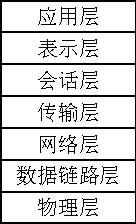
\includegraphics{graph/osi-1.pdf}
    \caption{OSI七层模型}
  \label{fig:osi}
\end{figure}

OSI参考模型有7层。适用于这7层的基本原则简要概括如下:\cite{computernetworks}
\begin{enumerate}[parsep=0pt]
\item 应该在需要一个不同抽象体的地方创建一层。
\item 每一层都应该执行一个明确定义的功能。
\item 每一层功能的选择应该向定义国际标准化协议的目标看齐。
\item 层与层边界的选择应该使跨越接口的信息流最小。
\item 层应该足够多,保证不同的功能不会被混杂在同一层,但同时层数不能太
  多,以免体系结构变得过于庞大。
\end{enumerate}

{\bfseries{物理层(physical layer):}}主要定义物理设备标准,如网线的接口
类型、光纤的接口类型、各种传输介质的传输率等。它的主要作用是传输比特
流\footnote{即由1、0转化为电流强弱来进行传输,到达目的地后再转化为1、0,
  也就是我们常说的数模转换与模数转换。}。这一层的数据叫做比特,网卡工作
在此层。一般物理层较少关心网络入侵分析,而更关注于保证设备的电缆安全。

{\bfseries{数据链路层(data link layer):}}主要将从物理层接收的数据进
行MAC地址(网卡的地址)的封装与解封装。这一层上的数据我们称为数据帧。在
这一层工作的设备是交换机,数据通过交换机来传输。

{\bfseries{网络层(network layer):}}主要将从下层收到的数据进行IP地址
的封装与解封装。在这一层工作的设备是路由器,我们称这一层的数据为数据包。

{\bfseries{传输层(transport layer):}}定义了一些传输数据的协议和端口
号,比如TCP\footnote{传输控制协议,传输效率低,可靠性强,用于传输可靠性
  要求高且数据量大的数据。}、UDP\footnote{用户数据报协议,与TCP的特性恰
  恰相反,用于传输可靠性要求不高且数据量小的数据。}。主要是将从下层接收
的数据进行分段,到达目的后进行数据重组。我们称这一层的数据为段。

{\bfseries{会话层(session layer):}}通过传输层(端口号:传输端口与接
收端口)建立数据传输的通路。主要在系统之间发起会话或接受会话请求(设备
之间可以通过IP,也可通过MAC或主机名来相互通信)。

{\bfseries{表示层(presentation layer):}}主要是接收的数据进行解释、加
密与解密、压缩与解压缩等(也就是把计算机能够识别的信息转化为人可以识别
的信息,如图片、声音等)。

{\bfseries{应用层(application layer):}}主要是一些终端应用,可把它理
解为应用层负责向用户或应用程序显示数据。

\subsection{TCP/IP三次握手}
\label{subsec:tcpIpThreeHandShake}

\subsection{TCP/IP四次挥手}
\label{subsec:tcpIpFourHandShake}

\chapter{H3C交换机配置}

\section{配置telnet方式登录}

\subsection{认证方式为Scheme时的登录配置}

\begin{verbatim}
sudo apt-get install git
sudo apt-get install git-core
\end{verbatim}

\section{以太网接口配置}

H3C交换机的配置如下:


配置方式与Cisco的很相似。

\begin{verbatim}
git config --global user.name "Laven Liu"
git config --global user.email "air.man.six@gmail.com"
\end{verbatim}

\subsection{打开或关闭以太网接口}
\label{sec:OpenShutInterface}

\begin{figure}[!htbp]
  \centering
  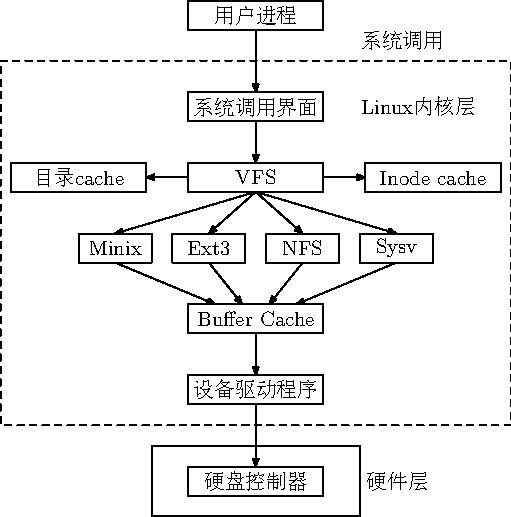
\includegraphics{graph/gnu-linux-0.pdf}
    \caption{Linux虚拟文件(测试图形)}
  \label{fig:LinuxVFS}
\end{figure}

\subsection{以太网端口基本属性配置}
\label{sec:BasicInterface}

\section{以太网接口的配置显示和维护}
